%!TEX root = ../rapport.tex

\chapter{Results}
\newcommand{\exampleheight}{2.2in}

The program implemented is able to draw illustrations of reduction graphs with
several different drawing algorithms. The algorithms output differs a lot, so
it can be beneficial to draw a graph multiple times with different algorithms.

% Screenshots!

\begin{figure}[htbp]
	% #a.(b) (#x.((x x) x) #y.((y y) y))
	\centering
	\subfigure[]{
		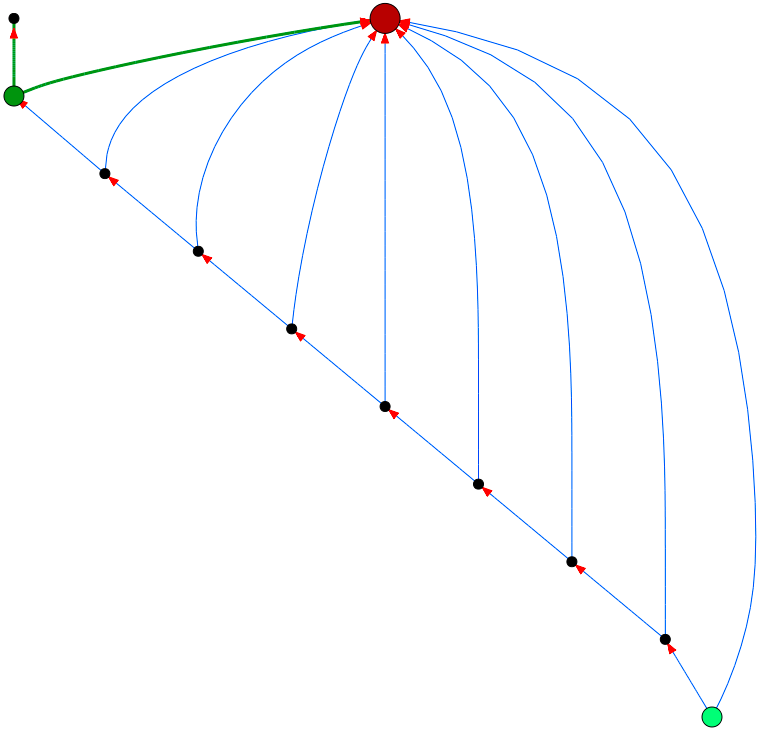
\includegraphics[height=\exampleheight]{../images/inf_reduction_graph_DOT.png}
	}
	\subfigure[]{
		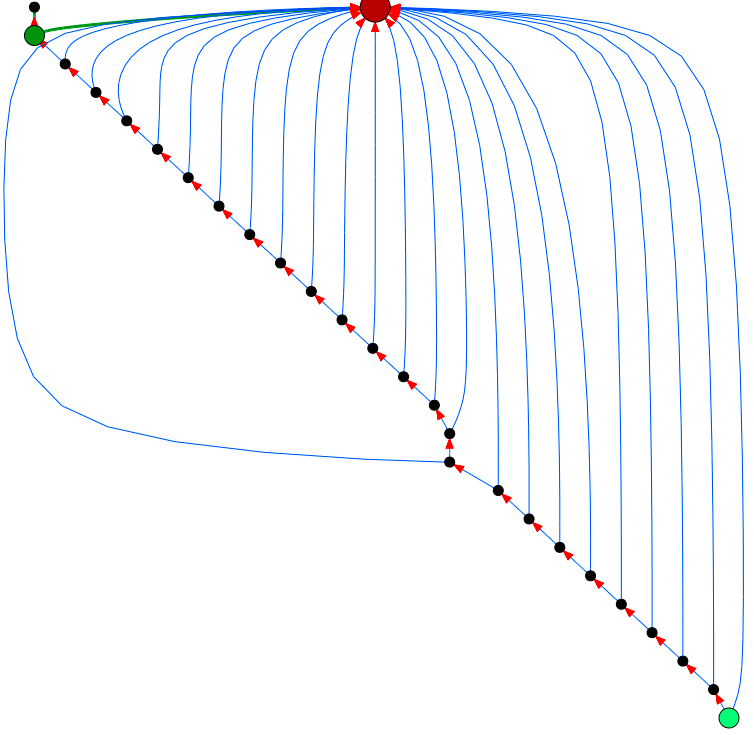
\includegraphics[height=\exampleheight]{../images/inf_reduction_graph_DOT2.png}
	}
	\caption{$G_\beta((\lam{a}{b}) (\lam{x}{(xxx)} \lam{y}{(yyy)}))$.}
	\label{fig:images_inf_reduction_graph_DOT}
\end{figure}

\begin{figure}[htbp]
	% #f.(#x.(f (x x))) (#x.(f (x x))) #y.((y y) y)
	\centering
	\subfigure[]{
		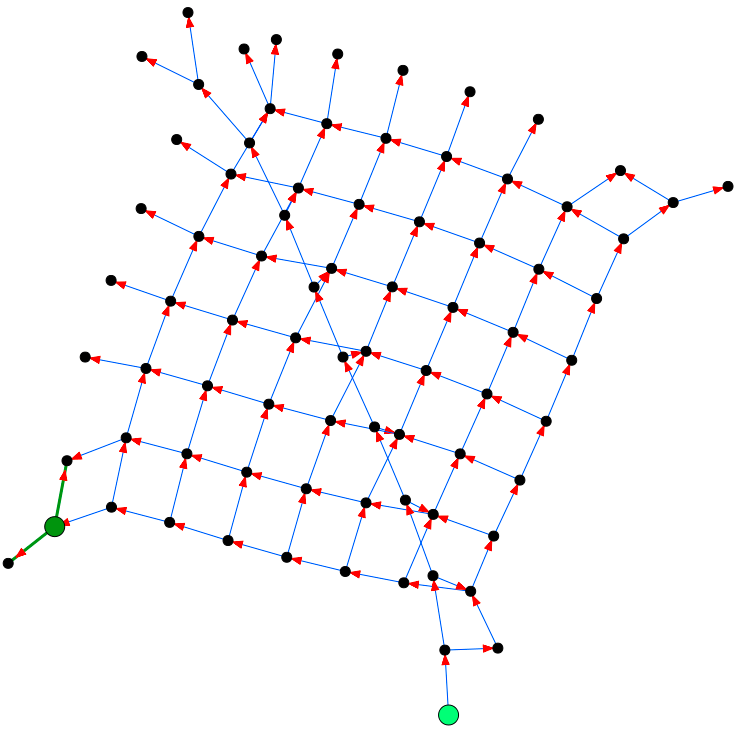
\includegraphics[height=\exampleheight]{../images/Ycomb_1_NEATO.png}
	}
	\subfigure[]{
		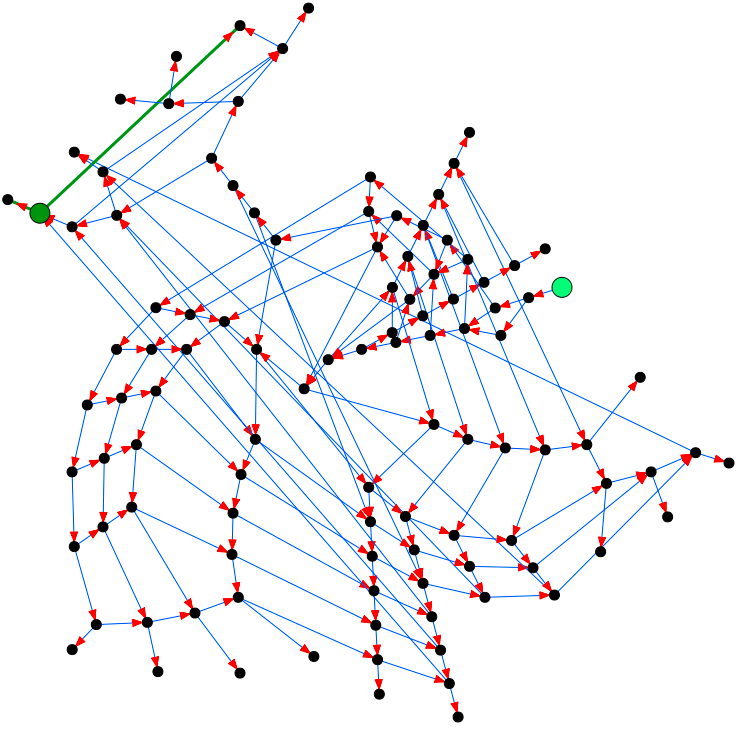
\includegraphics[height=\exampleheight]{../images/Ycomb_1_TWOPI.png}
	}
	\subfigure[]{
		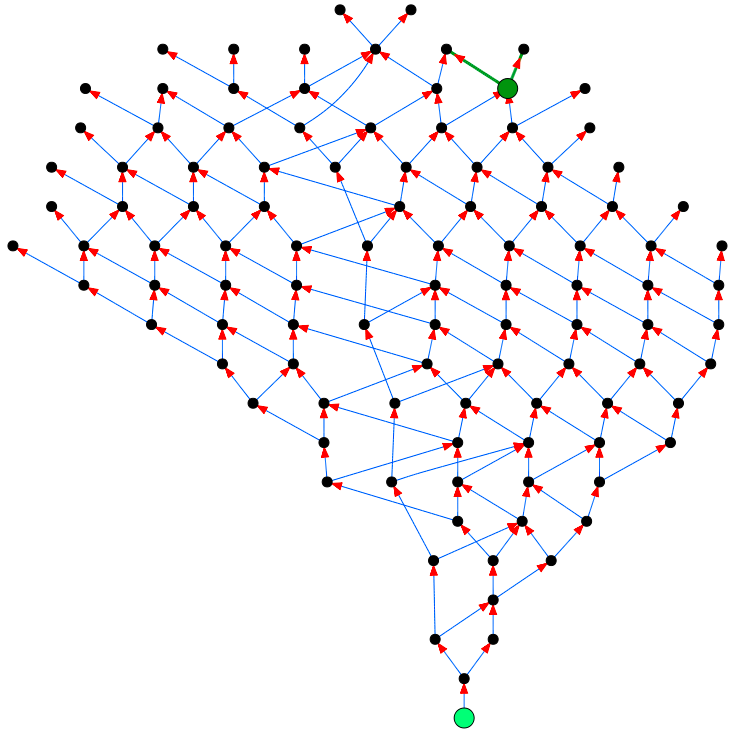
\includegraphics[height=\exampleheight]{../images/Ycomb_1_DOT.png}
	}
	\caption{$G_\beta((\lam{f}{(\lam{x}{f (x x)}) (\lam{x}{f (x x)})}) \lam{y}{(y y) y})$}
	\label{fig:images_inf_reduction_graph_DOT}
\end{figure}

\begin{figure}[htbp]
	% ((#b1.(b1) #b2.((#b3.(b2) #b4.((#b5.(b2) b4))))) #b6.((#b7.(b6) #b8.(#b9.(#b10.(#b11.(b11)))))))
	\centering
	\subfigure[Neato]{
		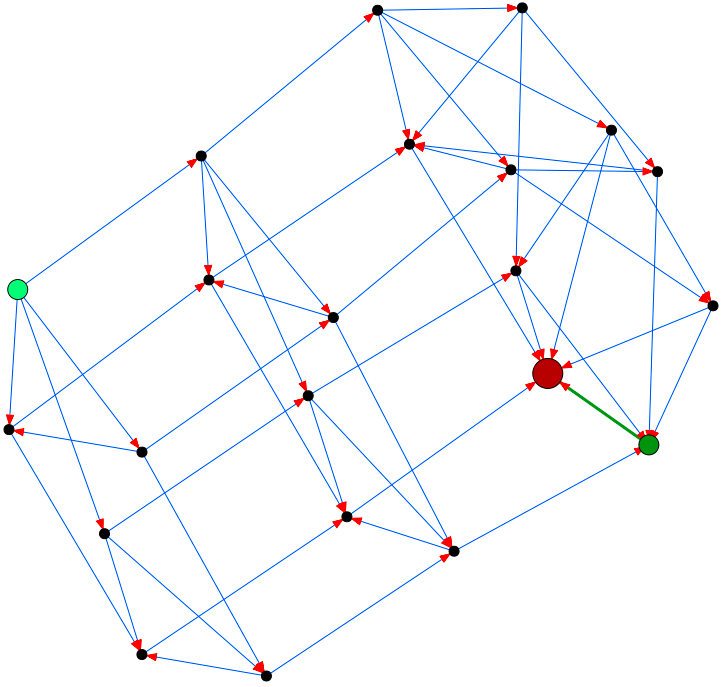
\includegraphics[height=\exampleheight]{../images/finite_ex_1_NEATO.png}
	}
	\subfigure[Dot]{
		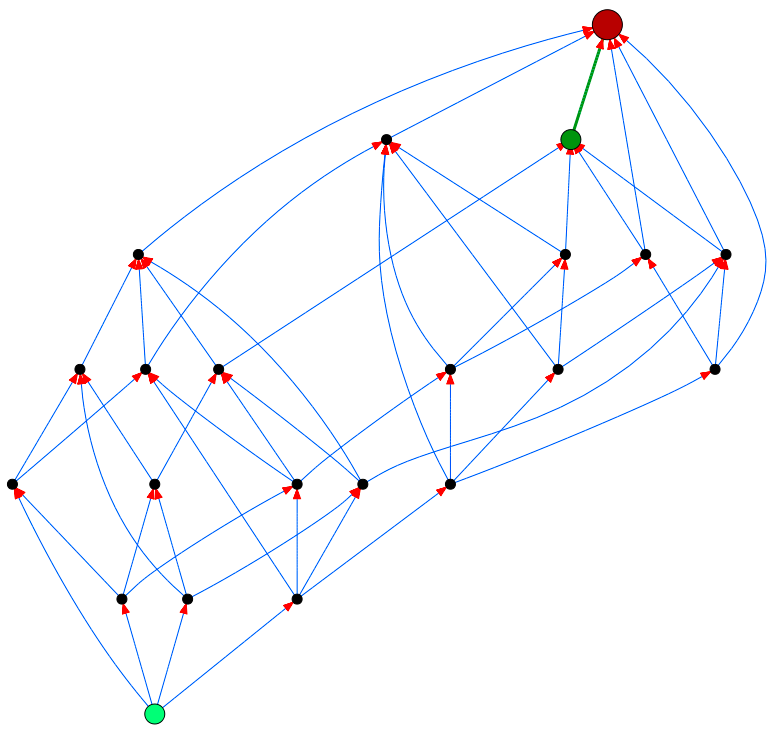
\includegraphics[height=\exampleheight]{../images/finite_ex_1_DOT.png}
	}
	\subfigure[Fdp]{
		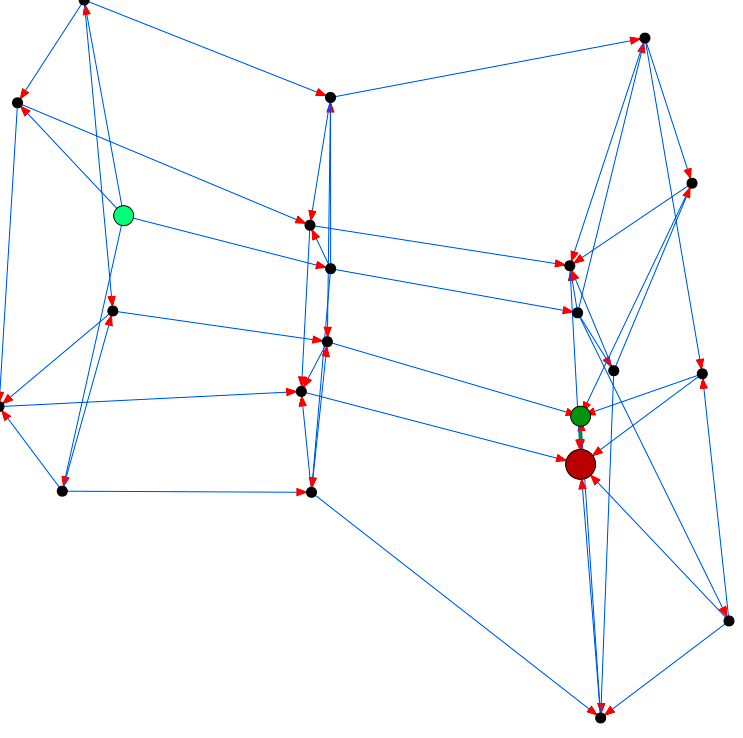
\includegraphics[height=\exampleheight]{../images/finite_ex_1_FDP.png}
	}

	\caption{$G_\beta\big(((\lam{x}{x}) \lam{y}{((\lam{z}{y}) \lam{z}{((\lam{a}{y}) z)})}) \lam{x}{((\lam{y}{x}) \lam{y}{(\lam{z}{(\lam{a}{\lam{b}{b}})})})}\big)$}
	\label{fig:images_finite_ex_1_NEATO}
\end{figure}

\begin{figure}[htbp]
	% (#B1.(#B2.(((#B3.(#B4.(#B5.(#B6.(B1)))) #B7.(#B8.(B7))) (#B9.(B1) #B10.(#B11.(B1)))))) (#B12.(#B13.(B13)) #B14.(#B15.(#B16.((#B17.(B17) B16))))))
	\renewcommand{\exampleheight}{2.5in}
	\centering
	\subfigure[Twopi]{
		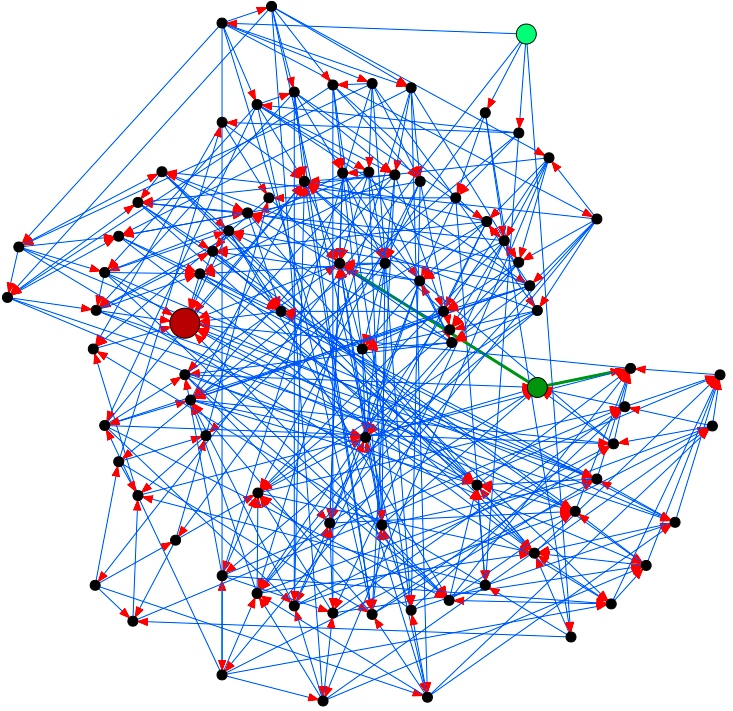
\includegraphics[height=\exampleheight]{../images/finite_ex_2_TWOPI.png}
	}
	\subfigure[Circo]{
		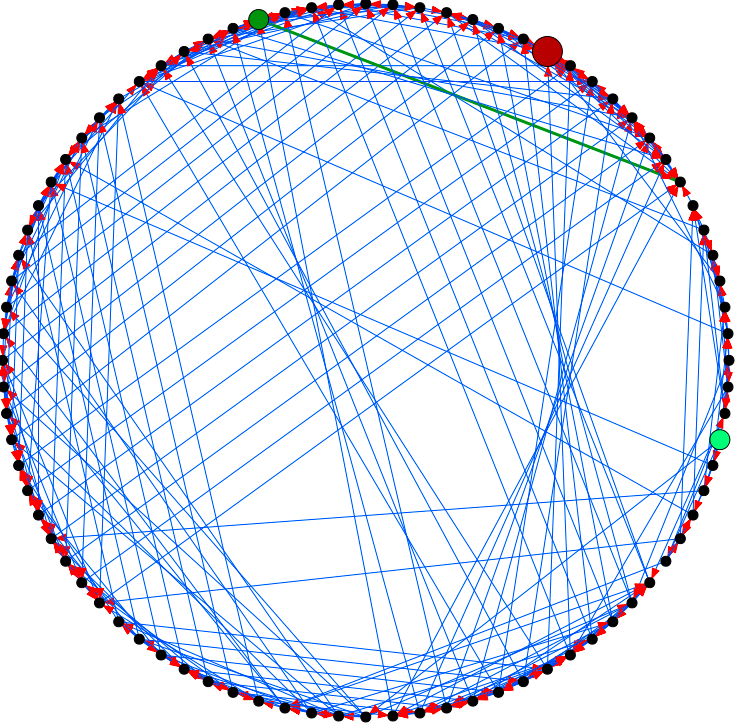
\includegraphics[height=\exampleheight]{../images/finite_ex_2_CIRCO.png}
	}
	\subfigure[Dot]{
		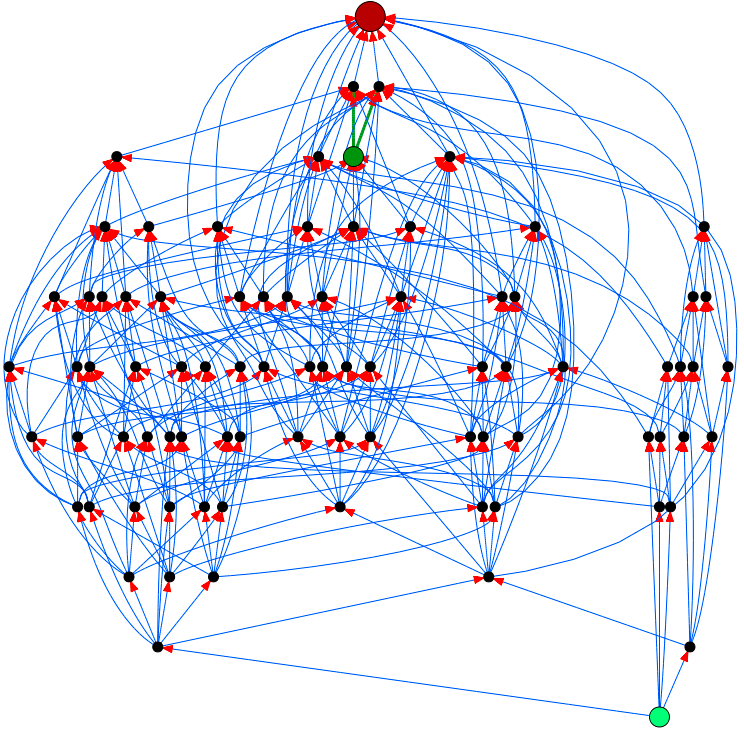
\includegraphics[height=\exampleheight]{../images/finite_ex_2_DOT.png}
	}
	\subfigure[Fdp]{
		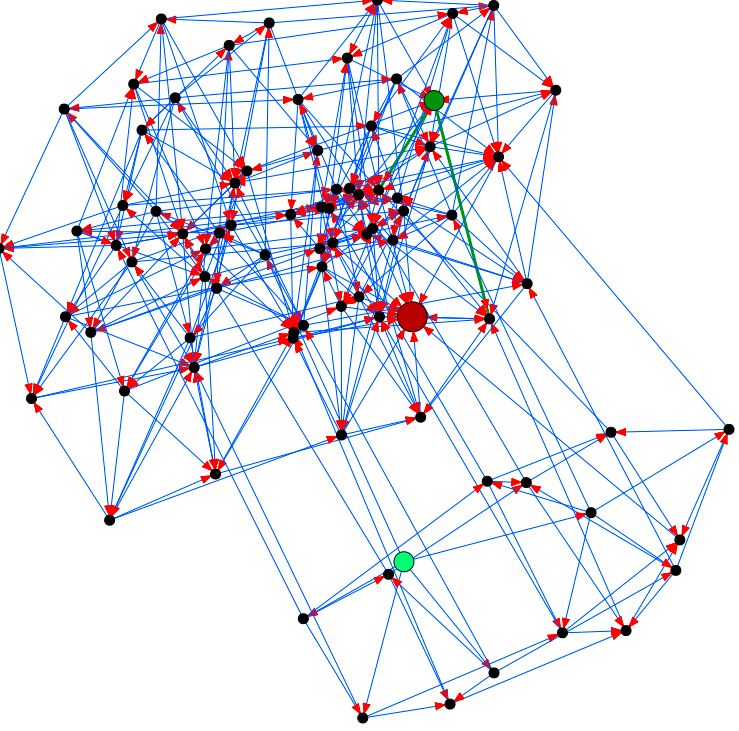
\includegraphics[height=\exampleheight]{../images/finite_ex_2_FDP.png}
	}
	\subfigure[Neato]{
		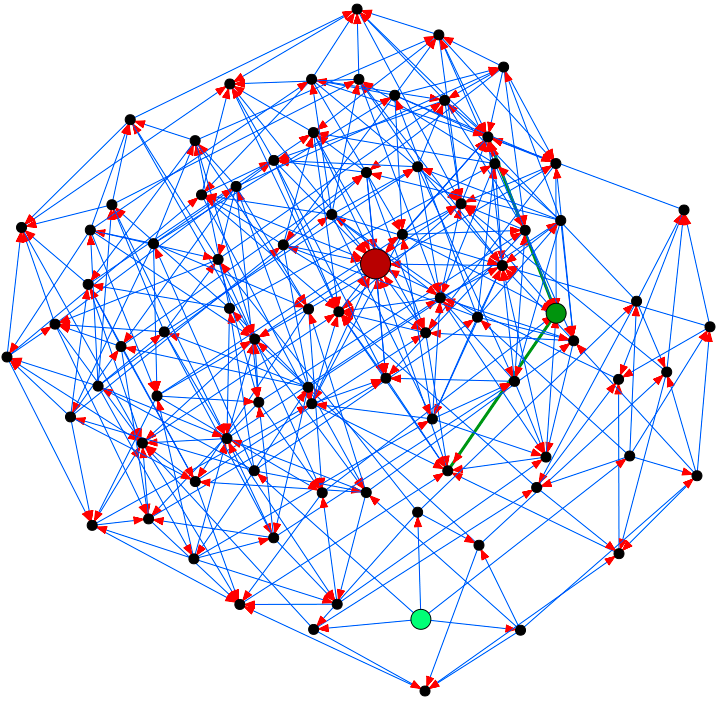
\includegraphics[height=\exampleheight]{../images/finite_ex_2_NEATO.png}
	}
	\subfigure[Majorization]{
		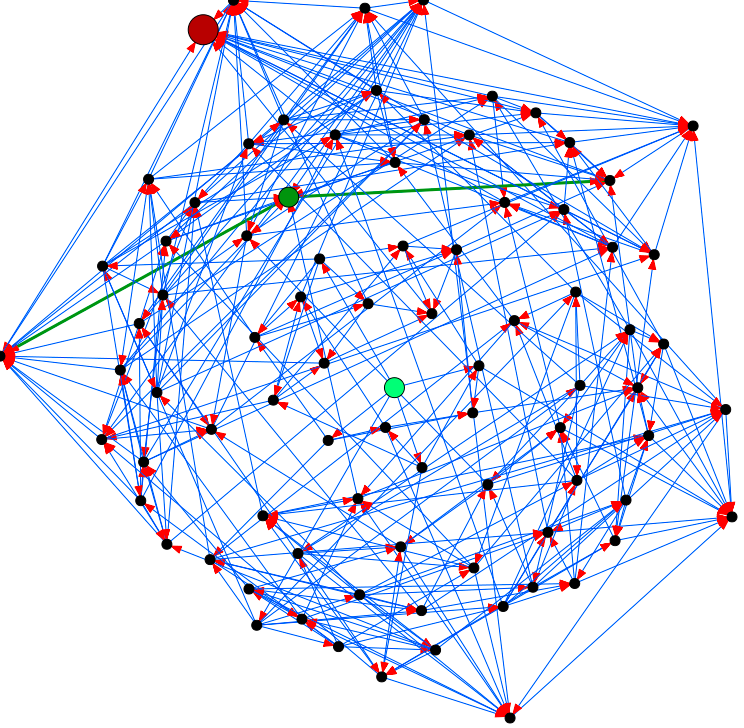
\includegraphics[height=\exampleheight]{../images/finite_ex_2_MAJOR.png}
	}
	
	\caption{$G_\beta\big(
	\lambda x.(\lambda y.((\lambda z.(\lambda a.(\lambda b.(\lambda c.x))) \lambda z.(\lambda a.z)) (\lambda y.x \lambda z.(\lambda a.x))
	)) (\lambda x.(\lambda y.y) \lambda x.(\lambda y.(\lambda z.(\lambda a.(a) z))))
	\big)$}
	\label{fig:images_finite_ex_2_CIRCO}
\end{figure}

% λB1.(((B1 λB2.(B1)) λB3.((λB4.((λB5.(λB6.(λB7.(B6))) ((B3 (λB8.(B3) λB9.(λB10.(B10)))) λB11.(B1)))) ((B3 B3) (B3 λB12.((B1 ((B3 λB13.(λB14.(B3))) ((λB15.(B3) λB16.(λB17.(λB18.(B17)))) λB19.(λB20.(B20))))))))))))

% λB1.((λB2.(λB3.((B2 F1))) λB4.(λB5.(((λB6.((B1 λB7.(B7))) λB8.((B4 λB9.(B4)))) λB10.(B10))))))



\begin{figure}[htbp]
	% λB1.((λB2.(λB3.((λB4.((B4 (λB5.(B1) λB6.(λB7.(B7))))) λB8.(B8)))) B1))
	\centering
	\subfigure[Majorization]{
		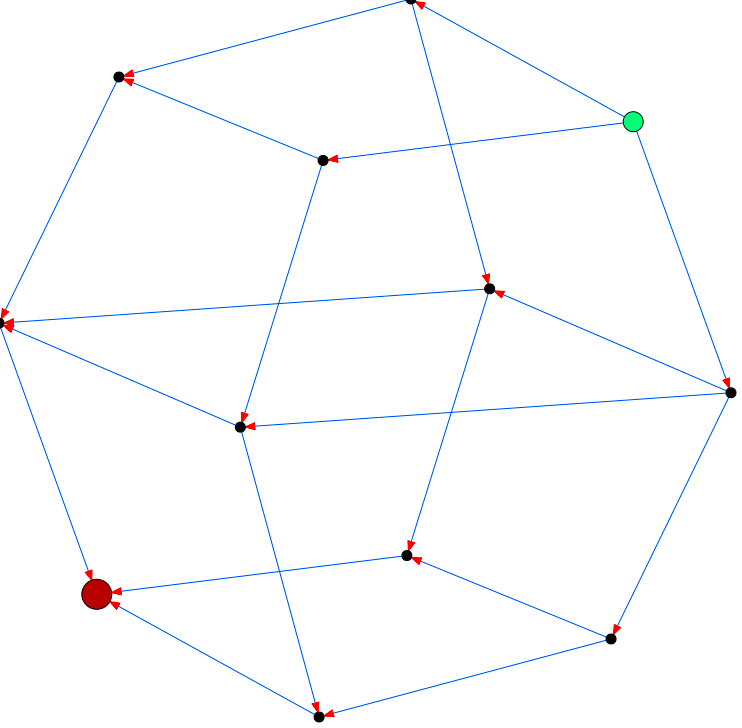
\includegraphics[height=\exampleheight]{../images/finite_ex_3_MAJOR.png}
	}
	\subfigure[Neato]{
		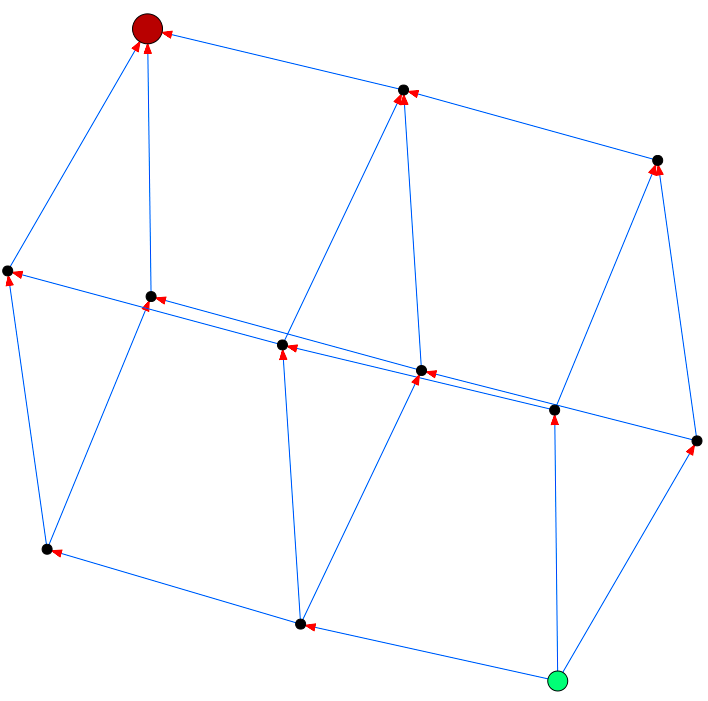
\includegraphics[height=\exampleheight]{../images/finite_ex_3_NEATO.png}
	}
	
	\caption{$G_\beta\big(\lambda x.(\lambda y.(\lambda z.(\lambda a.(a ((\lambda b.x) (\lambda c.\lambda d.d))) \lambda e.e)) x)\big)$}
	\label{fig:images_finite_ex_3_MAJOR}
\end{figure}

\begin{figure}[htbp]
	% #f.(#x.(f (x x))) (#x.(f (x x))) #y.(y y)
	\centering
	\subfigure[Circo]{
		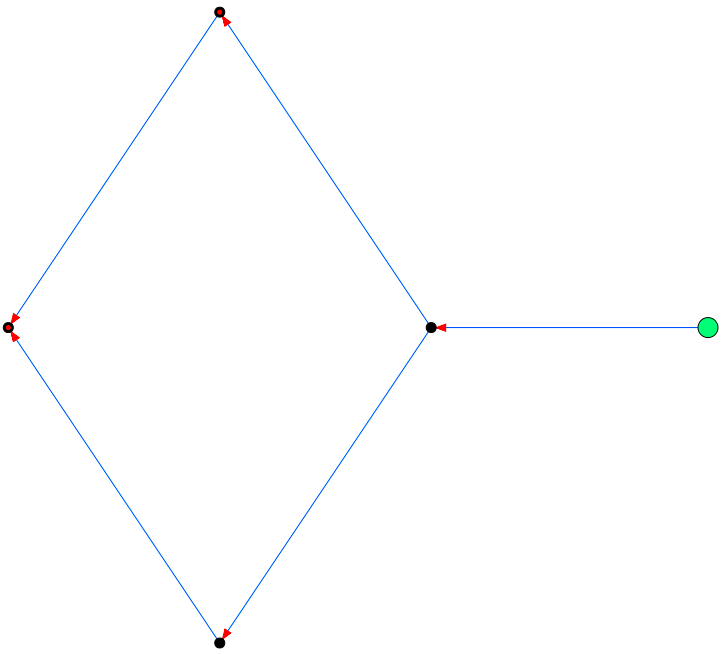
\includegraphics[height=\exampleheight]{../images/Ycomb_2_CIRCO.png}
	}
	\subfigure[Majorization]{
		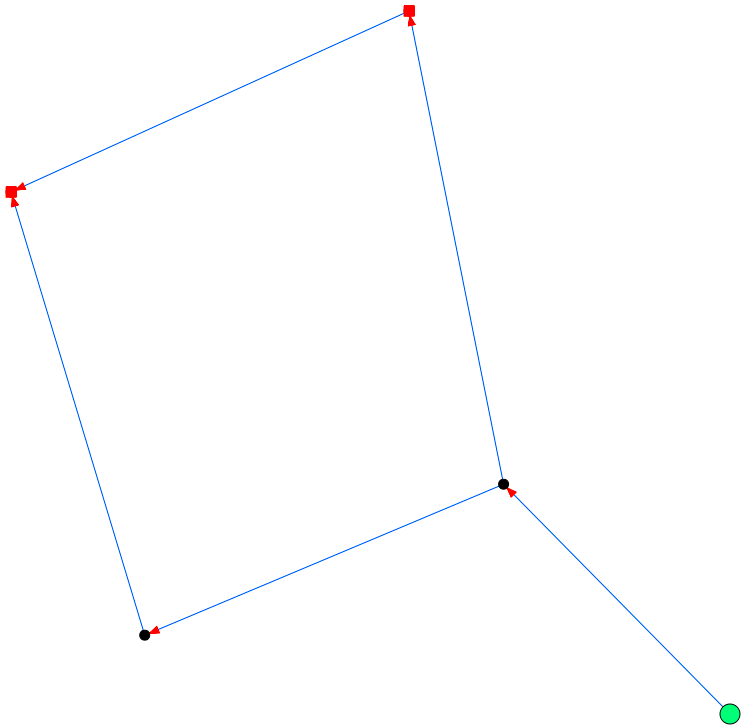
\includegraphics[height=\exampleheight]{../images/Ycomb_2_MAJOR.png}
	}
	
	\caption{caption}
	\label{fig:images_Ycomb_2_CIRCO}
\end{figure}
\begin{figure}[htbp]
	% #f.(#x.(f (x x))) (#x.(f (x x))) #x.#y.(y y x)
	\centering
	\subfigure[Majorization]{
		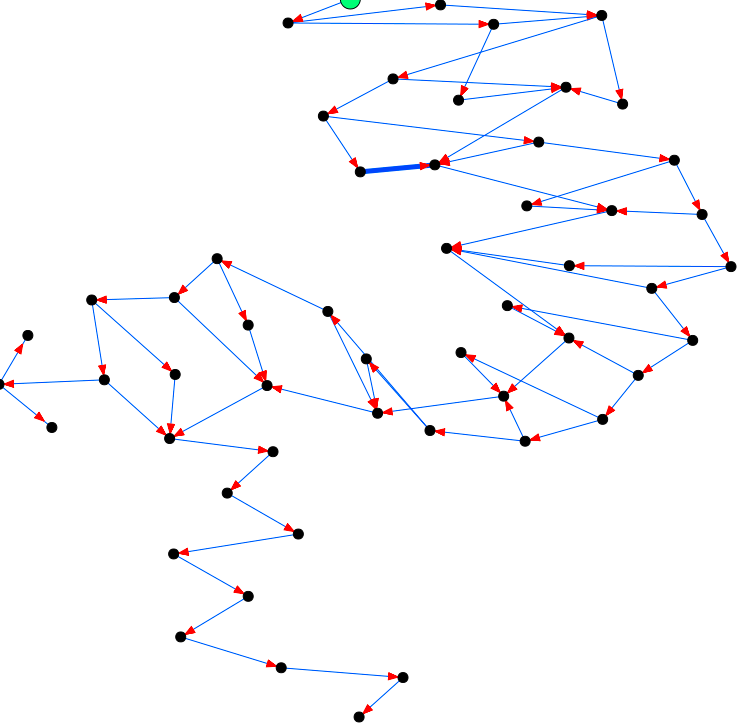
\includegraphics[height=\exampleheight]{../images/Ycomb_3_MAJOR.png}
	}
	\subfigure[Majorization, after more generations.]{
		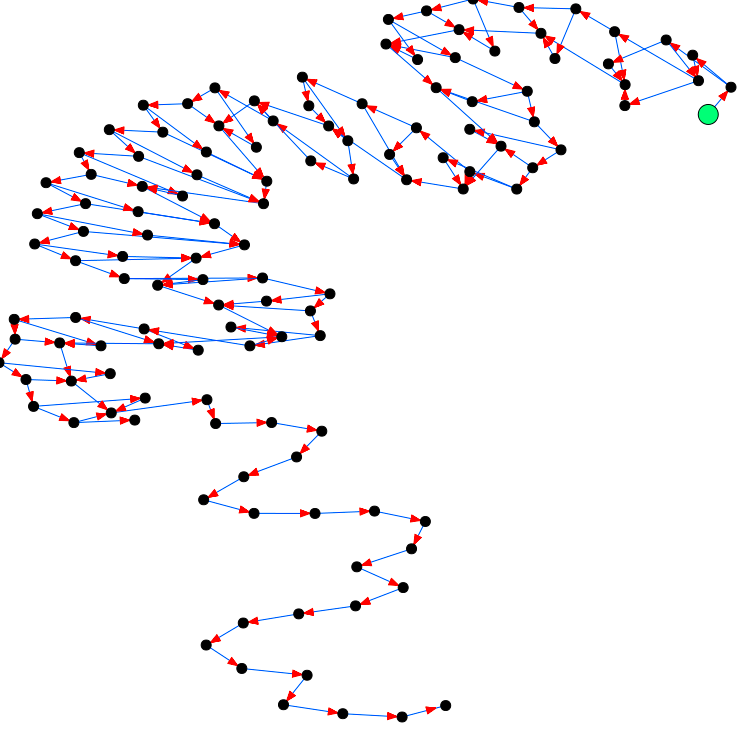
\includegraphics[height=\exampleheight]{../images/Ycomb_3_MAJOR2.png}
	}
	\subfigure[Neato]{
		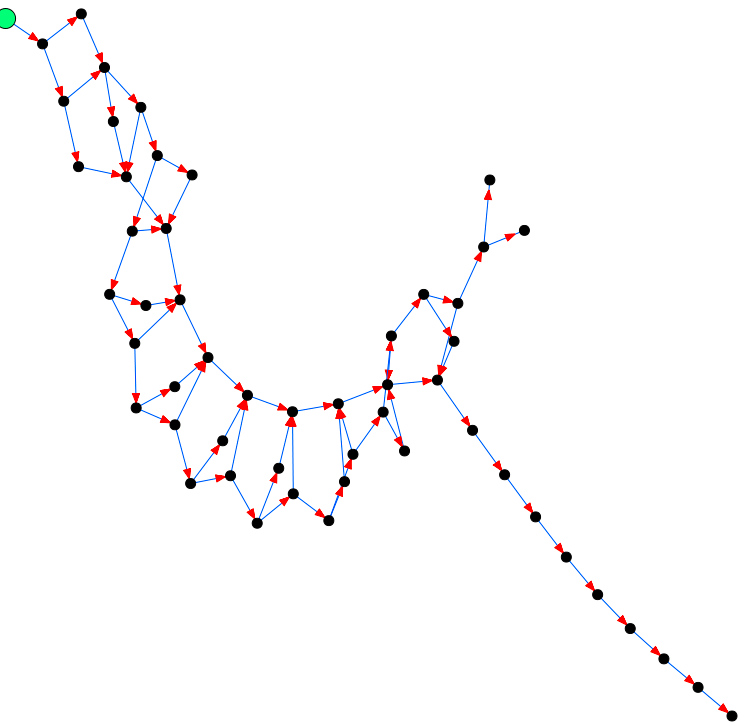
\includegraphics[height=\exampleheight]{../images/Ycomb_3_NEATO.png}
	}
	\subfigure[Neato, after more generations.]{
		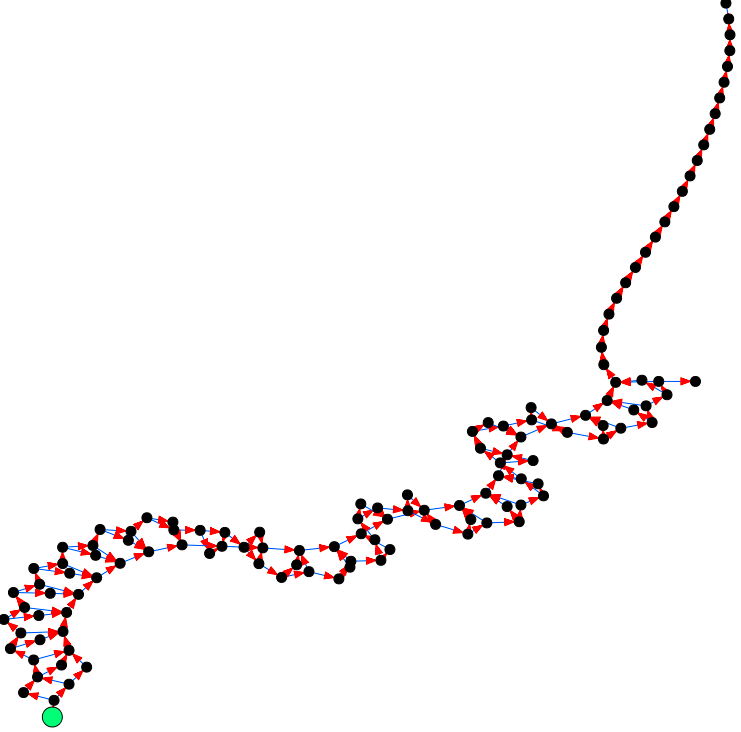
\includegraphics[height=\exampleheight]{../images/Ycomb_3_NEATO2.png}
	}
	\subfigure[Circo]{
		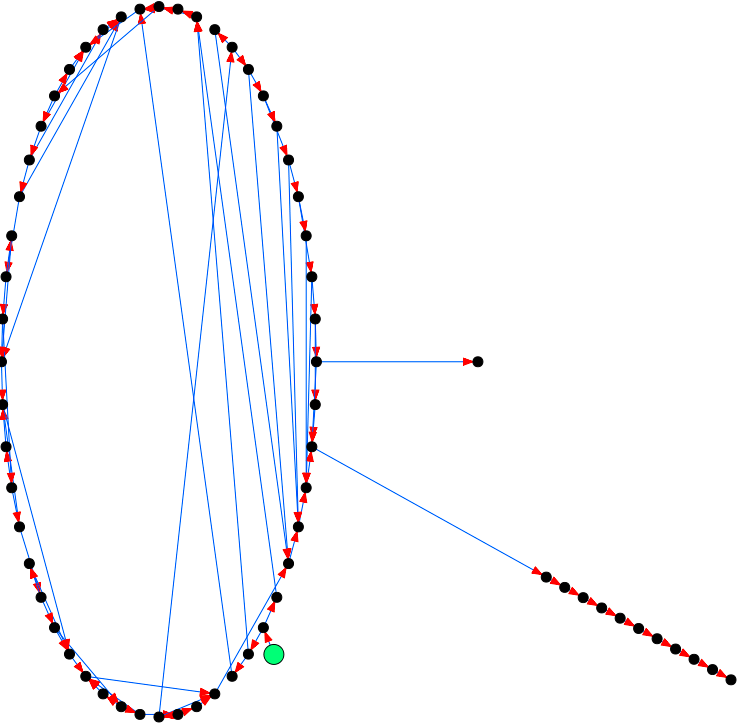
\includegraphics[height=\exampleheight]{../images/Ycomb_3_CIRCO.png}
	}
	\subfigure[Circo one step further; the lone outlier node emits new pairs of nodes.]{
		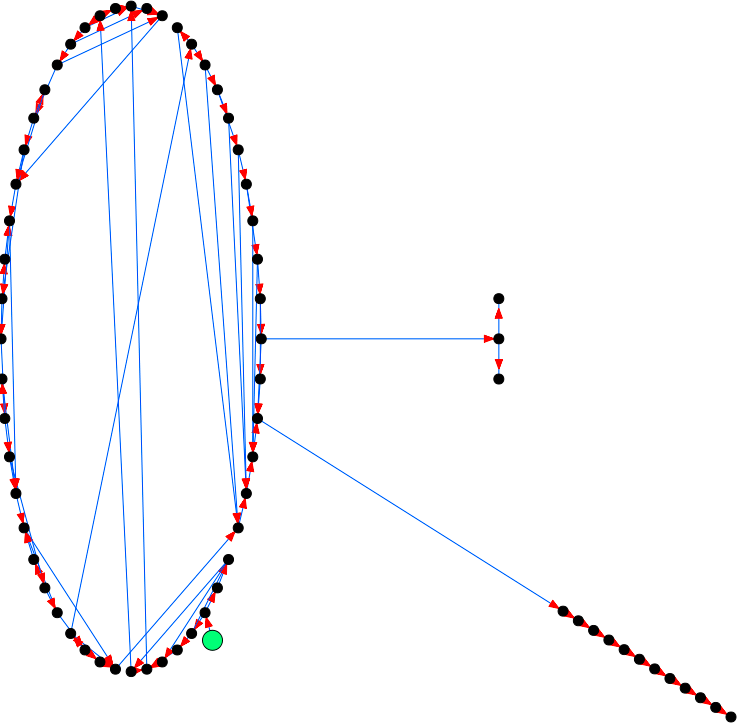
\includegraphics[height=\exampleheight]{../images/Ycomb_3_CIRCO2.png}
	}
	
	\caption{$G_\beta\big(\lambda f.\lambda x.(f (x x)) (\lambda x.f (x x)) \lambda x.\lambda y.(y y x)\big)$}
	\label{fig:images_Ycomb_3_DOT}
\end{figure}

\begin{figure}[htbp]
	% #f.(#x.(f (x x))) (#x.(f (x x))) #x.#y.(y y x)
	\centering
	\subfigure[Dot]{
		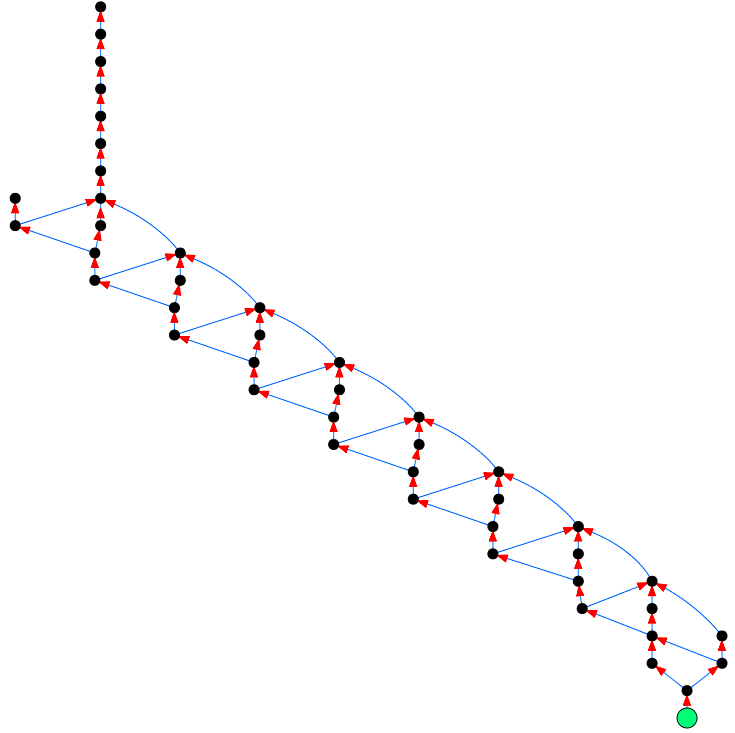
\includegraphics[height=\exampleheight]{../images/Ycomb_3_DOT.png}
	}
	\subfigure[Dot, after more generations.]{
		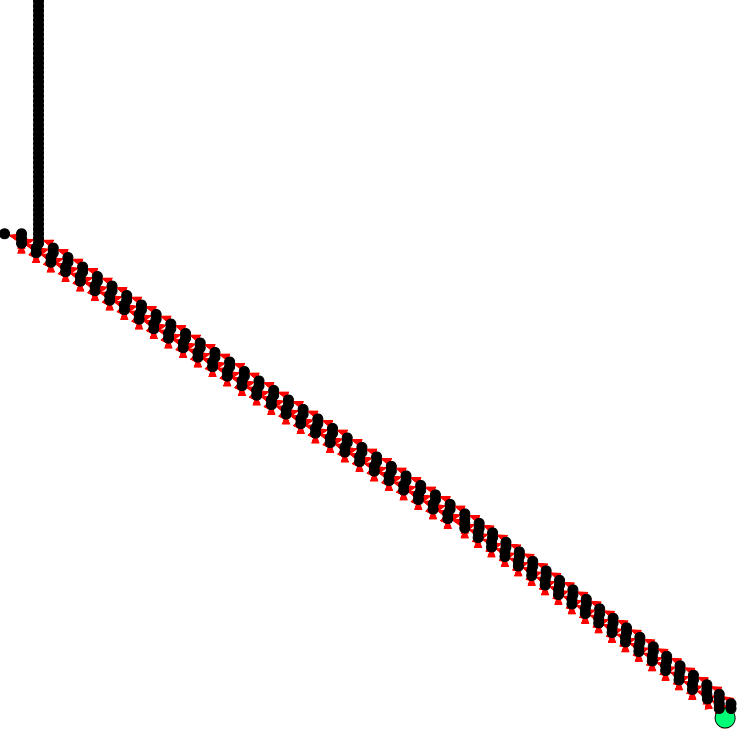
\includegraphics[height=\exampleheight]{../images/Ycomb_3_DOT2.png}
	}
	\subfigure[Fdp]{
		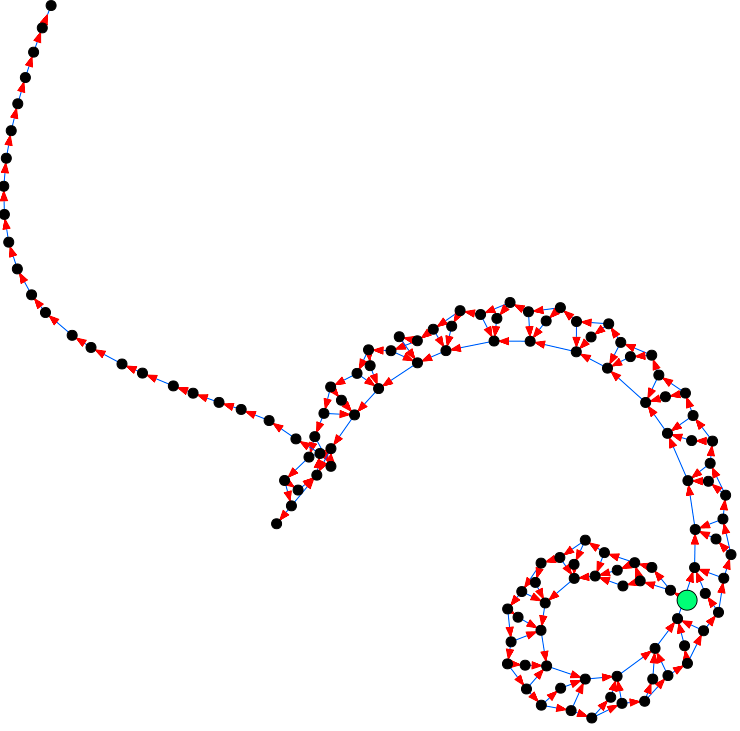
\includegraphics[height=\exampleheight]{../images/Ycomb_3_FDP.png}
	}
	\subfigure[Fdp, after more generations.]{
		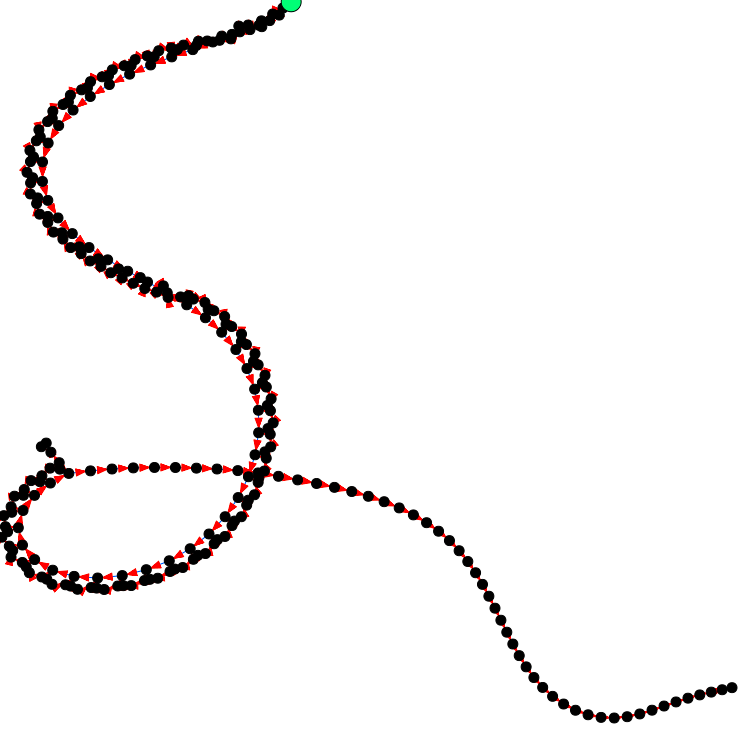
\includegraphics[height=\exampleheight]{../images/Ycomb_3_FDP2.png}
	}
	\subfigure[Twopi]{
		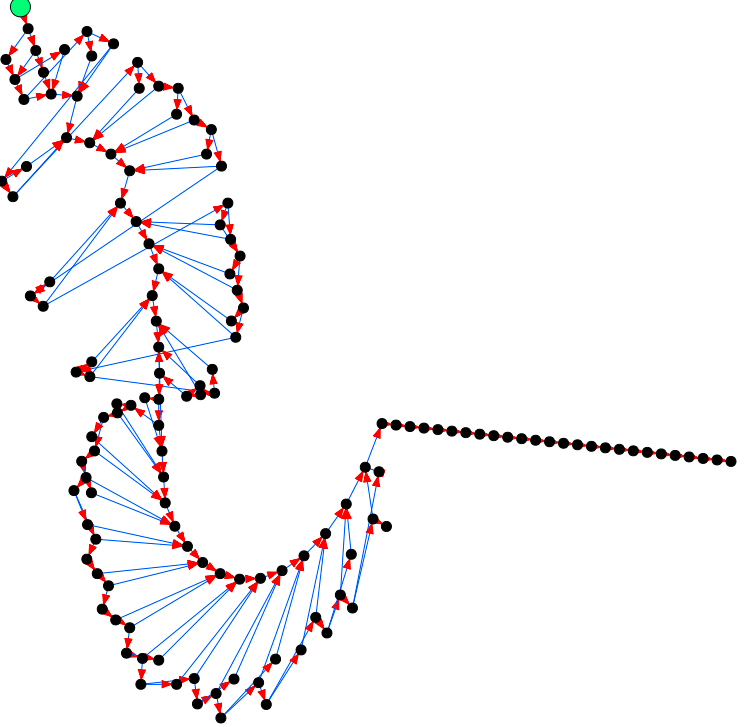
\includegraphics[height=\exampleheight]{../images/Ycomb_3_TWOPI.png}
	}
	\subfigure[Twopi, after more generations.]{
		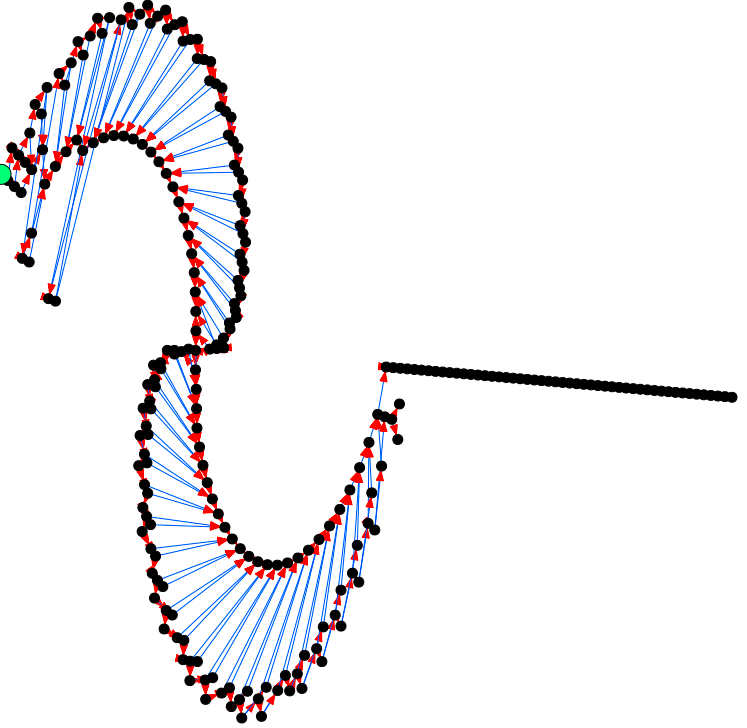
\includegraphics[height=\exampleheight]{../images/Ycomb_3_TWOPI2.png}
	}
	
	\caption{$G_\beta\big(\lambda f.\lambda x.(f (x x)) (\lambda x.f (x x)) \lambda x.\lambda y.(y y x)\big)$}
	\label{fig:images_Ycomb_3_DOT}
\end{figure}


% #x.(x x) #x.((x x) (x x))
% #x.(#y.(x y) #y.(x y)) #x.(x x) #x.(a)
% #f.(#x.(f (x x))) (#x.(f (x x))) #x.#y.(y (x y))